
% ===========================================================================
% file: vignette.rnw
% description: 
% requires: 
% author: Sahil Shah <sahil.shah@u.northwestern.edu>
% ==========================================================================

% LaTeX preamble and Top matter ----------------------------------------------

\documentclass[11pt]{article}
\usepackage[margin=0.9in]{geometry}
\usepackage{graphicx, amsmath, url,courier,array,csquotes}

\usepackage{Sweave}
\setkeys{Gin}{width=1.0\textwidth}
\graphicspath{{./}{figs/}}

\usepackage{hyperref}


%http://stackoverflow.com/questions/8902679/getting-sweave-code-chunks-inside-some-framed-box

\DefineVerbatimEnvironment{Sinput}{Verbatim} {xleftmargin=2em,
                                              frame=single}
\DefineVerbatimEnvironment{Soutput}{Verbatim}{xleftmargin=2em,
                                              frame=single}


\begin{document}

% =============================================================================

\title{\vspace{-1cm}The NIDG package Vignette}

\author{Sahil Shah and Rosemary Braun 
	   \href{mailto:rbraun@northwestern.edu}{<\texttt{rbraun@northwestern.edu}>}}

\date{\today}

\maketitle

% ----------------------------------------------------------------------------

\section*{Availability}  %------------------------------------------------

The \texttt{NIDG} package and its documentation are available on GitHub at 
\url{https://github.com/sahildshah1}. 


\section*{Introduction}  %------------------------------------------------

The \texttt{NIDG} package implements the method we previously developed~\cite{SHAH2017}
to identify disease-associated genes from expression data and an independent
network model of cellular interactions. We developed NIDG to find the genes
with neighbors on the network that are differentially expressed (with the
magnitude of the differential expression decreasing with distance from the
putative disease gene) and have correlated expression with the putative disease
gene. Since the differential expression of the neighbors of a putative disease
gene does not depend on their association with that gene, our algorithm consists
of two tests that are run independently of each other 
(Table~\ref{tab:procedure-sphere}, Table~\ref{tab:procedure-decay}). Their results
are then combined to determine if the putative disease gene is a central
candidate disease gene.

\section*{Example} %------------------------------------------------

In order to illustrate our method, we apply our algorithm  to one study  of
high-vs-low grade ovarian cancer  from the publicly available and curated
collection curatedOvarianData (GEO accession GSE14764)~\cite{Ganzfried2013}. We
have  constructed the global network model from KEGG
pathways~\cite{Kanehisa2008}.


\subsection*{Load Data Set} % --------------------------------------------


Our algorithm uses the correlation between the expression of the genes, their
differential expression, and their distances on the global network. 


\begin{Schunk}
\begin{Sinput}
> load("../../data/CurOvGradeKEGGnets.RData")
> load("../../data/largestCompKEGGigraph.RData")
> 
\end{Sinput}
\end{Schunk}


%figures-illustration.rnw but compute p-values instead of load 2016-04-06/geneNIDG.GSE14764.RData
%follow back geneNIDG.GSE14764 in 2016-04-06 in study.R etc to compute p-values

%<<fig=FALSE,echo=TRUE,width=11.43,height=6.71>>=

% # # GSE14764 -------------------------------------------------------------------
% # load("../../data/CurOv_RankCorMatrix_GSE14764_eset.RData")
% # load('../../data/CurOv_tStatistics.RData')

% # # LCC KEGGG -----------------------------------------------------------------
% # load("../../data/LCCKEGG_ShortestDistMatrix.RData")

% @


\subsection*{Source Functions} % ------------------------------------------

The functions that implement our method have to be sourced. The \texttt{Observed.SI,
Resample.SI,SumAbsCor} functions implement the \textit{Sphere of Influence} procedure
and the \texttt{Resample.DecayDE, Observed.DecayDE} functions implement the 
\textit{Decay of Differential Expression} procedure. The \texttt{geneNIDG}
function calls these functions. 


\begin{Schunk}
\begin{Sinput}
> library(pcaPP)
> library(igraph) # load largestCompKEGGigraph
> library(limma) #calcGeneStats()
> library(metap) #pFisher sumlog()
> source("../../R/calcCorMatrix.R")
> source("../../R/calcGeneTStats.R")
> source("../../R/calcAllPairsDistances.R")
> source("../../R/Observed.SI.R")
> source("../../R/Resample.SI.R")
> source("../../R/SumAbsCor.R")
> source("../../R/Resample.DecayDE.R")
> source("../../R/Observed.DecayDE.R")
> source("../../R/geneNIDG.R")
> 
\end{Sinput}
\end{Schunk}




\subsection*{Apply Functions to Data} % -----------------------------------



The correlation between the expression of the genes is calculated.


\begin{Schunk}
\begin{Sinput}
> CurOv_RankCorMatrix_GSE14764_eset <- 
+ calcCorMatrix(exprMatrix = CurOvGradeKEGGnets[["GSE14764_eset"]]$expr,
+ 			  corMethod = "spearman",
+ 			  exprName = paste("CurOvGradeKEGGnets$","GSE14764_eset",sep=""))
> 
\end{Sinput}
\end{Schunk}

% ---------------------------------------------------------------------------


The observed and resampled differential expression of the genes is calculated. 

\begin{Schunk}
\begin{Sinput}
> # List of observed (vector) and resampled (resampling by gene matrix) t statistics
> 
> intersectGeneNames = intersect(rownames(CurOvGradeKEGGnets[[2]]$expr),
+ 							   V(largestCompKEGGigraph)$name)
> expr = CurOvGradeKEGGnets[["GSE14764_eset"]]$expr
> classLabels = CurOvGradeKEGGnets[["GSE14764_eset"]]$grade
> #I can reduce the number of t tests by reducing the expr matrix to 
> #only genes that are on the network.
> reducedExpr = expr[intersectGeneNames,]
> geneTStats = calcGeneTStats(reducedExpr,
+ 							classLabels,
+ 							numResamples = 1000)
> 
\end{Sinput}
\end{Schunk}

% ---------------------------------------------------------------------------

The distances on the global network are calculated.


\begin{Schunk}
\begin{Sinput}
> CompKEGG_ShortestDistMatrix <- 
+ calcAllPairsDistances(network = largestCompKEGGigraph,
+ 					     directionPaths="all",
+ 					     weightVector = NULL,
+ 					     networkName = "largestCompKEGGigraph")
> 
\end{Sinput}
\end{Schunk}



In this example, MCM2 (KEGG ID: hsa:4171) is the candidate disease gene. 

\begin{Schunk}
\begin{Sinput}
> genes.assayedETnetwork <- intersect(
+ 	rownames(CurOv_RankCorMatrix_GSE14764_eset),
+ 	rownames(CompKEGG_ShortestDistMatrix))
> gene.id <- "hsa:4171"
> 
\end{Sinput}
\end{Schunk}


% ---------------------------------------------------------------------------



The Sphere of Influence and Decay of Differential Procedures are run.


\begin{Schunk}
\begin{Sinput}
> geneNIDG.hsa4171 <-  geneNIDG(
+ 	gene.id = gene.id,
+ 	distance.matrix = CompKEGG_ShortestDistMatrix,
+ 	cor.matrix = CurOv_RankCorMatrix_GSE14764_eset,
+ 	geneStats.observed = geneTStats$observed,
+ 	perm.geneStats.matrix = geneTStats$resampled,
+ 	num.Sphere.resamples = 1000,
+ 	diameter = 34,
+ 	genes.assayedETnetwork = genes.assayedETnetwork)
> 
> 
\end{Sinput}
\end{Schunk}

% ---------------------------------------------------------------------------


The evidence from both procedures is combined. 


\begin{Schunk}
\begin{Sinput}
> p.Fisher <- vapply( 1:34, function(index){
+ 
+ 	x <- sumlog( c(geneNIDG.hsa4171$p.Decay[index],
+ 			geneNIDG.hsa4171$p.Sphere[index]) )
+ 
+ 	return(x$p)
+ 
+ 
+ },
+ numeric(1) )
> geneNIDG.hsa4171 <- cbind(geneNIDG.hsa4171,p.Fisher)
> 
\end{Sinput}
\end{Schunk}
% ---------------------------------------------------------------------------




\subsection*{Description of the Output} % ---------------------------------



Our method outputs a data frame. 


\begin{Schunk}
\begin{Sinput}
> str(geneNIDG.hsa4171)
\end{Sinput}
\begin{Soutput}
'data.frame':	34 obs. of  8 variables:
 $ gene.id       : Factor w/ 1 level "hsa:4171": 1 1 1 1 1 1 1 1 1 1 ...
 $ radius        : int  1 2 3 4 5 6 7 8 9 10 ...
 $ size          : num  9 14 17 46 169 ...
 $ observed.tau_b: num  NaN -0.0156 -0.046 -0.4233 -0.0916 ...
 $ p.Decay       : num  1 0.509 0.426 0.003 0.106 0.019 0.667 0.219 0.145 0.131 ...
 $ observed.cor  : num  3.29 6.2 7.45 14.36 39.42 ...
 $ p.Sphere      : num  0.001 0.000999 0.000999 0.000999 0.000999 ...
 $ p.Fisher      : num  7.91e-03 4.36e-03 3.73e-03 4.11e-05 1.08e-03 ...
\end{Soutput}
\begin{Sinput}
> 
> 
\end{Sinput}
\end{Schunk}

% =======================================================================

We plot the results against every radius.

\begin{Schunk}
\begin{Sinput}
> source("../../R/plotRadiusVS.R")
> plotRadiusVS(geneNIDG.hsa4171)
> 
\end{Sinput}
\end{Schunk}
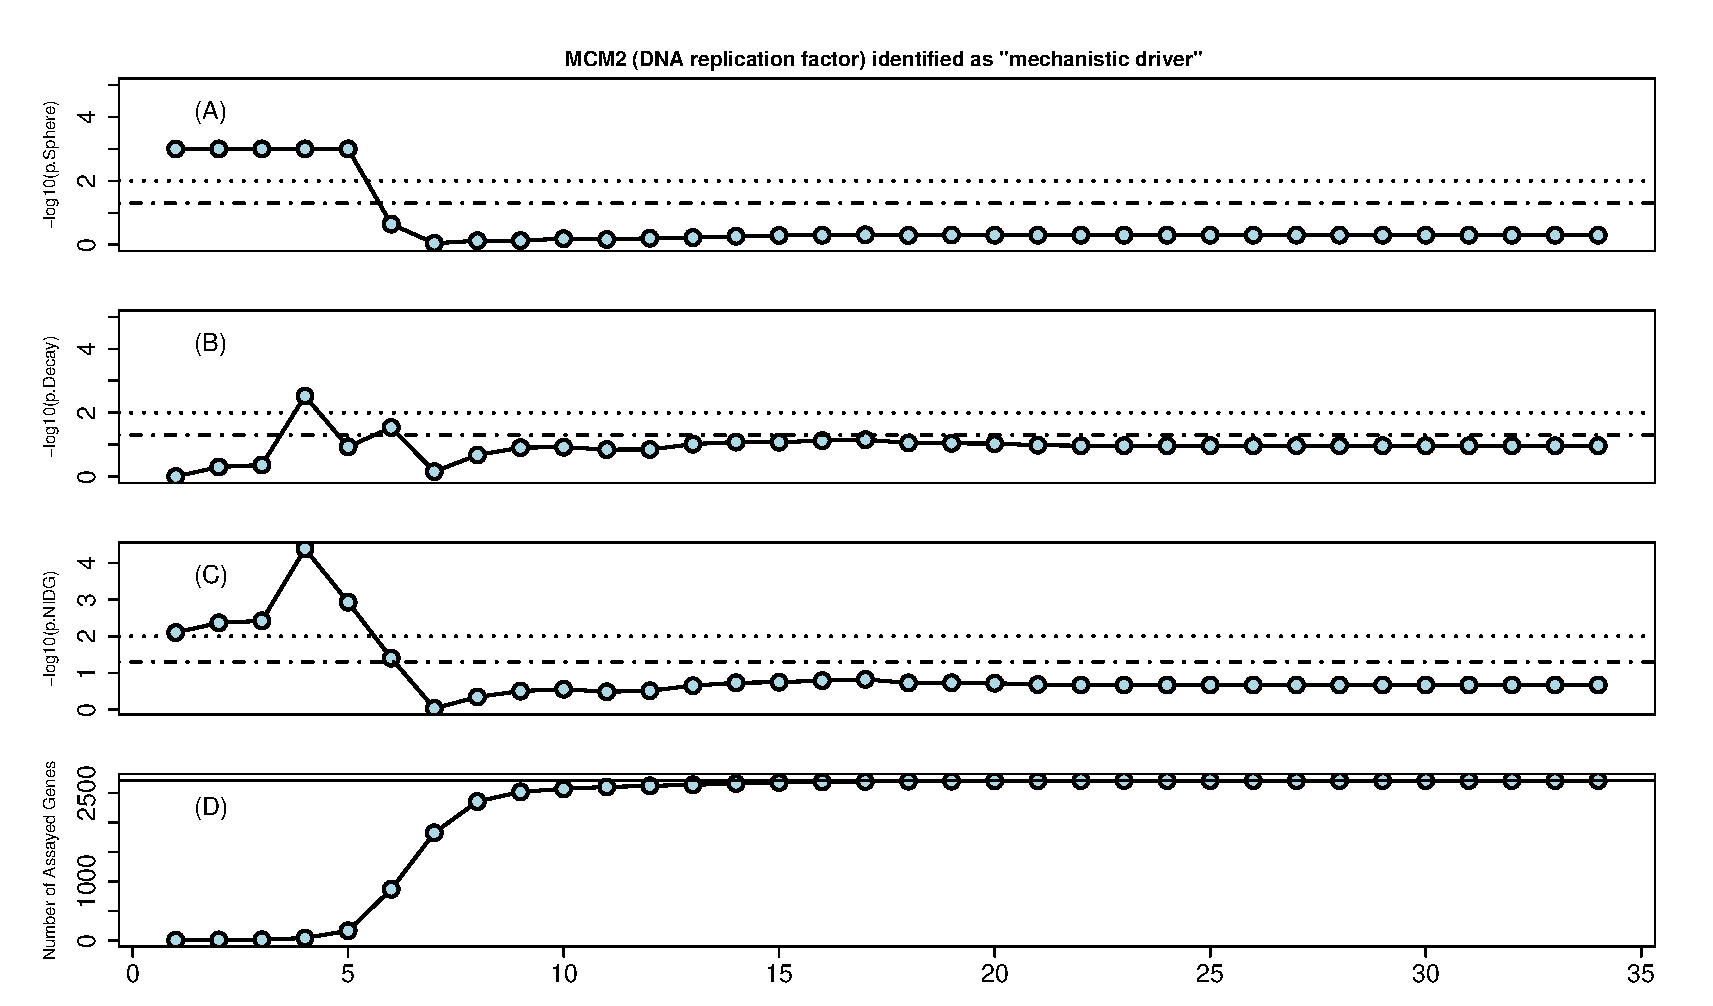
\includegraphics{vignette-main-010}



% \SweaveInput{vignette-radiusVSplots.rnw}


% =========================================================================

\clearpage

\subsection*{Tables}



\begin{table}[hb!]
\centering
  
\begin{tabular}{ p{\textwidth } }
  \hline
  
  \textbf{Sphere of Influence} \\
  \hline

 
  \begin{description}

    \item[\textbf{Input}]: Define the gene expression data and the network model

    \item[For] putative driver gene $i$ 

    \begin{enumerate}

        \item Calculate the Spearman rank correlation $\rho_k$ between the 
        	  expression of gene $k$ and gene $i$ across all the conditions
        	  in the expression matrix for every other gene $k$: 
            $\rho_1,\rho_2,\dots,\rho_{N-1}$
            (where $N$ is the number of genes both assayed and on the
            network)

       	\item Calculate the total observed correlation between gene $i$
       		  and its neighbors: $\sum_{k=1}^{M} |\rho_k|$ where the correlations
       		  $\rho_k$ are indexed so that the first $M$ genes are in the
       		  neighborhood of gene $i$

       	\item Compute the distribution of total correlation under the null by
       		    generating $N_{\text{Sphere}}$ null total correlations. To
              generate each null total correlation:

        \begin{enumerate}

            \item Bootstrap from the correlations calculated in Step (1)

            \item Preserve the gene indices's so that the first 
              re-sampled correlation is assigned to gene $k=1$, etc and
              recalculate the total correlation as in Step (2)

        \end{enumerate}


       	\item Compute $p^i_{\text{Sphere}}$ by counting the the proportion of 
       		  null sums greater than or equal to the observed sum. 
            If $p^i_{\text{Sphere}} = 0$, set 
       		  $p^i_{\text{Sphere}}=\frac{1}{N_\text{Sphere}+1}$


    \end{enumerate}


    \item[\textbf{Output}]: Return $p^i_{\text{Sphere}}$


  \end{description} \\
  
  \hline
\end{tabular}

\caption{The Sphere of Influence procedure tests if a putative driver gene
is more correlated with its network neighbors than with a random set of genes.}

\label{tab:procedure-sphere}
\end{table}




\begin{table}[hb!]
\centering
  
\begin{tabular}{ p{\textwidth } }
  \hline
  
  \textbf{Decay of Differential Expression} \\
  \hline

 
  \begin{description}

    \item[\textbf{Input}]: Define the gene expression data and the network model

    \item [Calculate] the moderated $t$-statistic $g_k$ between cases and
          controls of each gene: $g_1, g_2,\dots,g_{N}$
          % (where $N$ is the number of genes both assayed and on the network)

    \item[For] putative driver gene $i$ 

    \begin{enumerate}

    	\item Compute the observed discordance between differential expression and distance from gene $i$: $\tau_{B}( \{g_1,\dots,g_M\}, \{d(1,i),\dots,d(M,i)\}$
      where the gene-level statistics are indexed so that the first $M$ genes are in the neighborhood of gene $i$, $\tau_B$ is the Kendall rank correlation,
      and $d(k,i)$ is the geodesic distance between gene $k$ and gene $i$


      \item Compute the distribution of the discordance under the null by
      generating $N_{\text{Decay}}$ null discordances. To
      generate each null discordance:

      \begin{enumerate}

          \item Permute the phenotype labels and recalculate the moderated
          $t$-statistics for each gene

          \item Recompute the discordance as in Step (1)

      \end{enumerate}


      \item Compute $p^i_{\text{Decay}}$ by counting the the proportion of 
            null discordances less than or equal to the observed discordance. 
            If $p^i_{\text{Decay}} = 0$, set 
            $p^i_{\text{Decay}}=\frac{1}{N_\text{Decay}+1}$

    \end{enumerate}


    \item[\textbf{Output}]: Return $p^i_{\text{Decay}}$


  \end{description} \\
  
  \hline
\end{tabular}

\caption{The Decay of Differential Expression procedure tests if the discordance
between differential expression and distance from a putative driver gene is
greater with the phenotype labels we observe than with a random permutation 
of the labels.}

\label{tab:procedure-decay}
\end{table}



% Bibliography -------------------------------------------------------------

\clearpage
\bibliographystyle{unsrt}
% comma separated list:
\bibliography{main}




\end{document}
